Uma malha computacional pode ser estruturada ou não e 
a escolha do elemento que constitui esta malha é de vital
importância para uma boa precisão da solução. 
Alguns parâmetros podem influenciar na escolha de um
determinado grupo de elementos como por exemplo no caso onde existe uma condição
de restrição como é encontrada na equação Navier-Stokes devido
o forte acoplamento entre a velocidade e a pressão. Essa
restrição é conhecida como \textit{Babuska-Brezzi}
\cite{babuska1971}\cite{brezzi1974}.
Quando possuímos essa restrição, precisamos ter diferentes números de nós para cada
variável no mesmo elemento a fim de possuirmos estabilidade na
solução. Sendo assim, precisamos utilizar um \textit{elemento quadrático ou cúbico}.
Mas a formulação corrente-voticidade da equação Navier-Stokes não
possui a restrição \textit{Babuska-Brezzi} já que não há
o acoplamento entre a velocidade e a pressão. Desta forma,
o uso de um \textit{elemento linear} não produz instabilidade,
podendo ser utilizado sem problemas neste trabalho.

\medskip
Abaixo apresentaremos a classificação dos elementos quanto à geometria
e à ordem do polinômio interpolador conforme apresentado por Anjos (2007) \cite{anjos2007}:

\begin{itemize}
 \item Geometria
  \begin{itemize}
   \item problemas unidimensionais - Reta
   \item problemas bidimensionais - Triangulares e Retangulares 
   \item problemas tridimensionais - Tetraedrais, hexaedrais e prismáticos
  \end{itemize}
 \item Ordem do polinômio interpolador
  \begin{itemize}
   \item grau um - Linear
   \item grau dois - Quadrática
   \item grau três - Cúbica
  \end{itemize}
\end{itemize}

\medskip
Os elementos triangulares são os mais comuns no MEF porque possibilita
uma boa discretização de superfícies irregulares devido a sua 
simplicidade geométrica. Neste trabalho, utilizamos um elemento triangular
com o polinômio interpolador de ordem um, isto é, linear.

\vspace{0.5cm}
Abaixo são apresentados alguns elementos triangulares com
diferentes ordens do polinômio interpolador:

\medskip
\noindent
\textbf{Elemento triangular linear:} Devido sua simplicidade, é o elemento
mais utilizado em MEF quando não possuímos restrições. As matrizes elementares
analíticas deste elemento são facilmente encontradas na literatura. Como se trata
de um elemento linear, a ordem do polinômio interpolador é de grau um. Desta forma,
suas funções de interpolação são planas. 
Este elemento é representado pela \ref{elemento triangular linear}:

\begin{figure}[H]
\begin{center}
\begin{tikzpicture}[scale=3]
 \draw (0,0) -- (1,0) -- (0.5,1) -- cycle;

 \node[circle, fill=black, inner sep=0pt, minimum size=5pt,label=below left:{1}] at (0,0) {};
 \node[circle, fill=black, inner sep=0pt, minimum size=5pt,label=below right:{2}] at (1,0) {};
 \node[circle, fill=black, inner sep=0pt, minimum size=5pt,label=above:{3}] at (0.5,1) {};
 
 \node[draw=none, scale=1.2] at (2,0.5) {$N_i = L_i$};
 \node[draw=none, scale=1.2] at (3.2,0.5) {$i = 1,2,3$};
\end{tikzpicture}
\end{center}
\caption{Elemento triangular linear}
\label{elemento triangular linear}
\end{figure}

%\begin{figure}[H]
%  \centering
%  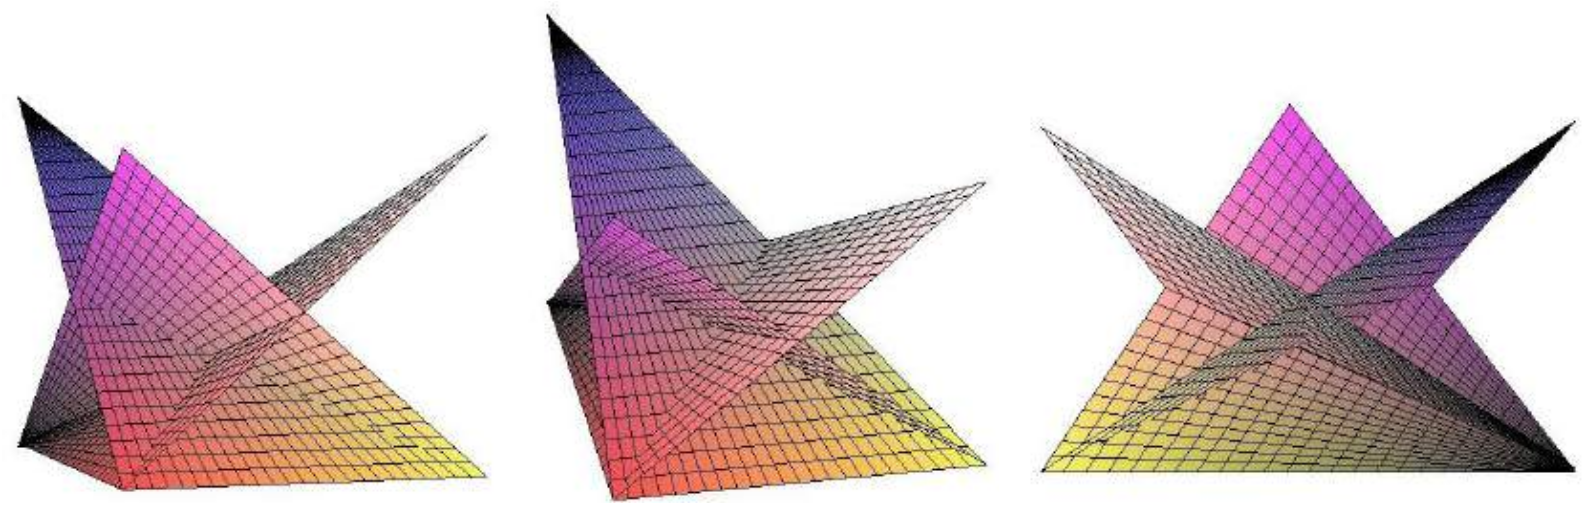
\includegraphics[scale=0.25]{./02_chaps/cap_mef/figure/tri_linear.png}
% \caption{Funções de Interpolação para o elemento triangular linear.}
% \label{tri_linear}
%\end{figure}


\medskip
\noindent
\textbf{Elemento triangular quadrático:} Geralmente este elemento é usado quando
possuímos restrições que impedem o uso do elemento linear ou quando estamos buscando uma
melhor aproximação do resultado. As matrizes elementares 
deste elemento são calculadas pela quadratura gaussiana cujos parâmetros podem ser
encontrados na literatura. Como se trata de um elemento quadrático, a ordem do polinômio 
interpolador é de grau dois. Desta forma, suas funções de interpolação são parabólicas.
Este elemento é representado pela \ref{elemento triangular quadrático}:

\begin{figure}[H]
\begin{center}
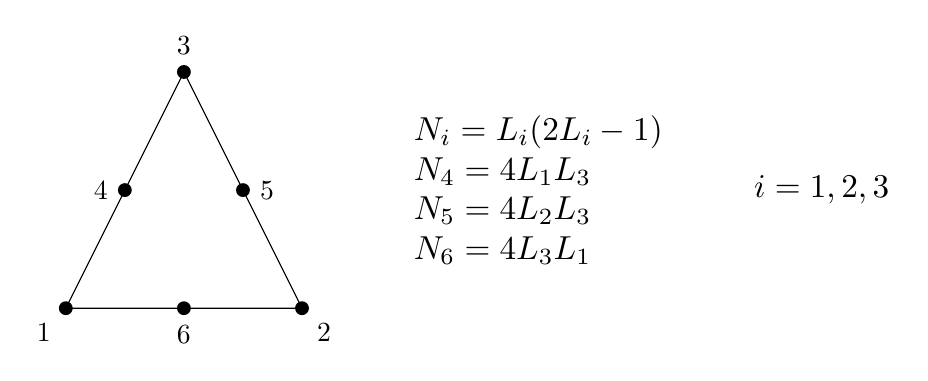
\begin{tikzpicture}[scale=3] 
 \draw (0,0) -- (1,0) -- (0.5,1) -- cycle;
 \node[circle, fill=black, inner sep=0pt, minimum size=5pt,label=below left:{1}] at (0,0) {};
 \node[circle, fill=black, inner sep=0pt, minimum size=5pt,label=below right:{2}] at (1,0) {};
 \node[circle, fill=black, inner sep=0pt, minimum size=5pt,label=above:{3}] at (0.5,1) {};
 \node[circle, fill=black, inner sep=0pt, minimum size=5pt,label=left:{4}] at (0.25,0.5) {};
 \node[circle, fill=black, inner sep=0pt, minimum size=5pt,label=right:{5}] at (0.75,0.5) {};
 \node[circle, fill=black, inner sep=0pt, minimum size=5pt,label=below:{6}] at (0.5,0.0) {};

 \node[draw=none, align=left, scale=1.2] at (2,0.5) {$N_i = L_i(2L_i - 1)$\\
                                                    $N_4 = 4L_1L_3$\\
                                                    $N_5 = 4L_2L_3$\\
                                                    $N_6 = 4L_3L_1$};

 \node[draw=none, scale=1.2] at (3.2,0.5) {$i = 1,2,3$};
\end{tikzpicture}
\end{center}
\caption{Elemento triangular quadrático}
\label{elemento triangular quadrático}
\end{figure}

\medskip
\noindent
\textbf{Elemento triangular cúbico:} Assim como o elemento quadrático, este elemento é usado quando
possuímos restrições que impedem o uso do elemento linear ou quando estamos buscando uma
melhor aproximação do resultado. Na literatura, este elemento é conhecido como \textit{elemento MINI}.
Suas matrizes elementares também são calculadas pela quadratura gaussiana. 
Como se trata de um elemento cúbico, a ordem do polinômio 
interpolador é de grau três. Desta forma, suas funções de interpolação possui
uma bolha no centro do elemento.
Este elemento é representado pela \ref{elemento triangular cúbico}:

\begin{figure}[H]
\begin{center}
\begin{tikzpicture}[scale=3] 
 \draw (0,0) -- (1,0) -- (0.5,1) -- cycle;
 \node[circle, fill=black, inner sep=0pt, minimum size=5pt,label=below left:{1}] at (0,0) {};
 \node[circle, fill=black, inner sep=0pt, minimum size=5pt,label=below right:{2}] at (1,0) {};
 \node[circle, fill=black, inner sep=0pt, minimum size=5pt,label=above:{3}] at (0.5,1) {};
 \node[circle, fill=black, inner sep=0pt, minimum size=5pt,label=above:{4}] at (1/2,1/3) {};
 
 \node[draw=none, align=left, scale=1.2] at (2,0.5) {$N_i = L_1 - 9L_1L_2L_3$\\
                                                    $N_4 = 27L_1L_2L_3$};

 \node[draw=none, scale=1.2] at (3.2,0.5) {$i = 1,2,3$};
\end{tikzpicture}
\end{center}
\caption{Elemento triangular cúbico}
\label{elemento triangular cúbico}
\end{figure}

%\begin{figure}[H]
%  \centering
%  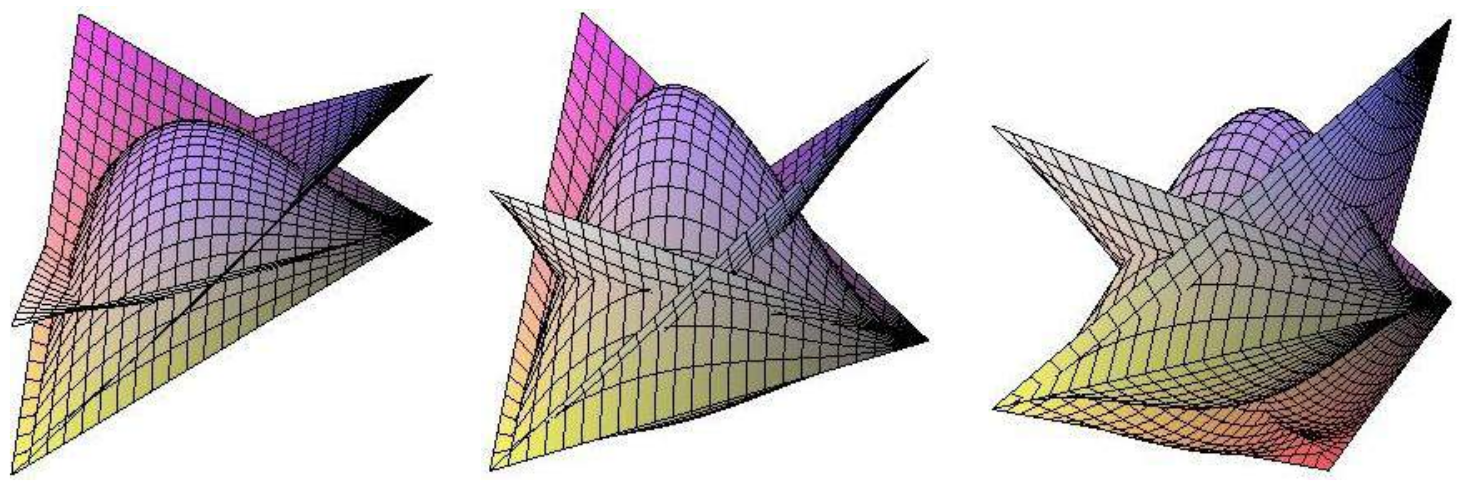
\includegraphics[scale=0.25]{./02_chaps/cap_mef/figure/mini.png}
% \caption{Funções de Interpolação para o elemento MINI.}
% \label{mini}
%\end{figure}

\medskip
\noindent
As Eqs (\ref{vorticity pre matrix} a \ref{concentration pre matrix}) podem ser representadas matricialmente por:

\begin{equation}
\begin{aligned}
 M \overset{.}{w} + u \cdot G_x w  + v \cdot G_y w & + \frac{1}{\textit{Re}} \Big[ K_{xx} + K_{yy} \Big] w
 \\[5pt]
 & + \frac{\Delta t}{2} u \Big[ u K_{xx} + v K_{yx} \Big] w 
 + \frac{\Delta t}{2} v \Big[ u K_{xy} + v K_{yy} \Big] w 
 = 0 \label{vorticity matrix}
\end{aligned}
\end{equation}

\begin{equation}
 - \Big[ K_{xx} + K_{yy} \Big] \psi + Mw = 0
\end{equation}

\begin{equation}
 Mu - G_y \psi = 0
\end{equation}

\begin{equation}
 Mv + G_x \psi = 0
\end{equation}

\begin{equation}
\begin{aligned}
 M \overset{.}{c} + u \cdot G_x c + v \cdot G_y c & + \frac{1}{\textit{ReSc}} \Big[ K_{xx} + K_{yy} \Big] c
 \\[5pt]
 & + \frac{\Delta t}{2} u \Big[ u K_{xx} + v K_{xy} \Big] c
 + \frac{\Delta t}{2} v \Big[ u K_{yx} + v K_{yy} \Big] c 
 = 0 \label{concentration matrix}
\end{aligned} 
\end{equation}

\medskip
\noindent
onde as matrizes \textbf{M}, \textbf{G\textsubscript{x}}, 
\textbf{G\textsubscript{y}}, \textbf{K\textsubscript{xx}},
\textbf{K\textsubscript{xy}},
\textbf{K\textsubscript{yx}}, 
\textbf{K\textsubscript{yy}}, 
possuem dimensões \textbf{np} x \textbf{np}
(isto é, número de nós por número de nós) e
são definidas como:

\begin{align}
  \textbf{M} & = \textbf{A} m^{e}\\
  \textbf{G\textsubscript{x}} & = \textbf{A} g_{x}^{e}\\
  \textbf{G\textsubscript{y}} & = \textbf{A} g_{y}^{e} \\
  \textbf{K\textsubscript{xx}} & = \textbf{A} k_{xx}^{e} \\
  \textbf{K\textsubscript{xy}} & = \textbf{A} k_{xy}^{e} \\
  \textbf{K\textsubscript{yx}} & = \textbf{A} k_{yx}^{e} \\
  \textbf{K\textsubscript{yy}} & = \textbf{A} k_{yy}^{e}
\end{align}

\noindent
onde \textbf{A} é um operador de montagem das
matrizes elementares nas matrizes globais, 
respeitando a correspondência entre os índices
globais e locais e 
$m^{e}$, 
$g^{e}_{x}$,
$g^{e}_{y}$,
$k^{e}_{xx}$,
$k^{e}_{xy}$,
$k^{e}_{yx}$,
$k^{e}_{yy}$
são as matrizes elementares cuja dimensão para o 
\textit{elemento triangular linear} é \textit{3}x\textit{3} e 
são definidas por:


\begin{equation}
 \begin{aligned}
  m^{e} & = \int_{\Omega^{e}} N_{i}^{e} N_{j}^{e} d\Omega \\
  g_{x}^{e} & = \int_{\Omega^{e}} \frac{\partial N_{i}^{e}}{\partial x} N_{j}^{e} d\Omega \\
  g_{y}^{e} & = \int_{\Omega^{e}} \frac{\partial N_{i}^{e}}{\partial y} N_{j}^{e} d\Omega \\
  k_{xx}^{e} & = \int_{\Omega^{e}} \frac{\partial N_{i}^{e}}{\partial x} \frac{\partial N_{j}^{e}}{\partial x} \\
  k_{xy}^{e} & = \int_{\Omega^{e}} \frac{\partial N_{i}^{e}}{\partial x} \frac{\partial N_{j}^{e}}{\partial y} \\
  k_{yx}^{e} & = \int_{\Omega^{e}} \frac{\partial N_{i}^{e}}{\partial y} \frac{\partial N_{j}^{e}}{\partial x} \\
  k_{yy}^{e} & = \int_{\Omega^{e}} \frac{\partial N_{i}^{e}}{\partial y} \frac{\partial N_{j}^{e}}{\partial y}
 \end{aligned}
\end{equation}

\medskip
Sendo assim, as equações de governo em sua forma matricial discretizadas
segundo o Método dos Elementos Finitos que usamos neste trabalho foram:

\begin{equation} \label{final equation}
\begin{aligned}
 \frac{M}{\Delta t} w^{n+1} = \frac{M}{\Delta t} w^{n} - u \cdot G_x w^{n} & - v \cdot G_y w^{n} 
 - \frac{1}{\textit{Re}} \Big[ K_{xx} + K_{yy} \Big] w^{n}  
 \\[5pt]
 & - \frac{\Delta t}{2} u \Big[ u K_{xx} + v K_{yx} \Big] w^{n} 
 - \frac{\Delta t}{2} v \Big[ u K_{xy} + v K_{yy} \Big] w^{n} 
\end{aligned}
\end{equation}


\begin{equation}
 \Big[ K_{xx} + K_{yy} \Big] \psi = Mw
\end{equation}

\begin{equation}
 Mu = G_y \psi
\end{equation}

\begin{equation}
 Mv = - G_x \psi
\end{equation}

\begin{equation}
\begin{aligned}
 \frac{M}{\Delta t} c^{n+1} = \frac{M}{\Delta t} c^{n}  - u \cdot G_x c^{n} - v & \cdot G_y c^{n} 
 - \frac{1}{\textit{ReSc}} \Big[ K_{xx} + K_{yy} \Big] c^{n}  
 \\[5pt]
 & - \frac{\Delta t}{2} u \Big[ u K_{xx} + v K_{yx} \Big] c^{n} 
 - \frac{\Delta t}{2} v \Big[ u K_{xy} + v K_{yy} \Big] c^{n} 
\end{aligned}
\end{equation}
